\documentclass[../../../../main.tex]{subfiles}
\begin{document}

\begin{flushright}
\footnotesize\textit{【自動文字起こし・要確認】}
\end{flushright}

\noindent
[\textbf{解}] $y_1 = f(x) = \frac{\pi}{4}\frac{1}{x} - \frac{\pi}{4} + 1$, $y_2 = g(x) = \sqrt{2}\cos \frac{\pi}{4}x$ とおく。

\begin{enumerate}
    \item[(1)] $y_1 - y_3 = \frac{\pi}{4}\frac{1}{x} - \frac{\pi}{4} + 1 - \frac{\pi}{4} + \frac{\pi}{4}x - 1 = \frac{\pi}{4}\left(x + \frac{1}{x} - 2\right)$ であり, $0 < x \le 1$ では
    AM-GMから
    \[
    y_1 - y_3 \ge \frac{\pi}{4}(2-2) = 0
    \]
    等号成立は $x=1$ $\dots \text{①}$

    $y_3 - y_2 = \frac{\pi}{4}(1-x) + 1 - \sqrt{2}\cos\frac{\pi}{4}x$
    \[
    = \frac{\pi}{4}(1-x) + \sqrt{2}\left(\cos\frac{\pi}{4} - \cos\frac{\pi}{4}x\right)
    \]
    これは $x=1$ で等号成立。 $0 < x < 1$ の時, 平均値の定理から
    \[
    \cos\frac{\pi}{4} - \cos\frac{\pi}{4}x = (1-x) \cdot \left(-\frac{\pi}{4}\right) \sin\frac{\pi}{4}c \quad (0 < c < 1)
    \]
    をみたす $c$ があるので
    \[
    y_3 - y_2 = \frac{\pi}{4}(1-x)\left[ 1 - \sqrt{2}\sin\frac{\pi}{4}c \right] > 0 \quad (\because \sqrt{2}\sin\frac{\pi}{4}c < 1)
    \]
    だから, ②とあわせて
    \[
    y_3 \ge y_2 \quad (\text{等号成立は } x=1) \quad \dots \text{②}
    \]
    ①, ②から, $0 < x < 1$ では $y_1 > y_2$ となり, 交点を持たず, $x=1$ での $(1,1)$ のみである．(終)

    \item[(2)] 右図から, もとめる面積 $S$ として
    \[
    \begin{aligned}
    S &= \int_0^{1/2} \left(1 + \frac{\pi}{4} - \sqrt{2}\cos\frac{\pi}{4}x\right) dx + \int_{1/2}^1 (f(x) - g(x)) dx \\
    &= \int_0^{1/2} \left(1 + \frac{\pi}{4}\right) dx + \int_{1/2}^1 f(x) dx - \int_0^1 g(x) dx \quad \dots \text{③}
    \end{aligned}
    \]
    ここで,
    \begin{itemize}
        \item $\int_0^{1/2} \left(1 + \frac{\pi}{4}\right) dx = \frac{1}{2}\left(1 + \frac{\pi}{4}\right)$
        \item $\int_{1/2}^1 f(x) dx = \left[ \frac{\pi}{4}\log x + \left(1-\frac{\pi}{4}\right)x \right]_{1/2}^1 = \frac{\pi}{4}\log 2 + \frac{1}{2}\left(1-\frac{\pi}{4}\right)$
        \item $\int_0^1 g(x) dx = \sqrt{2} \frac{4}{\pi} \left[ \sin\frac{\pi}{4}x \right]_0^1 = \frac{4}{\pi}$
    \end{itemize}
    を③に代入して
    \[
    \begin{aligned}
    S &= \frac{1}{2}\left(1+\frac{\pi}{4}\right) + \frac{\pi}{8}\log 2 + \frac{1}{2}\left(1-\frac{\pi}{4}\right) + \frac{4}{\pi} \\
    &= 1 + \frac{4}{\pi} + \frac{\pi}{8}\log 2
    \end{aligned}
    \]
\end{enumerate}

\begin{center}
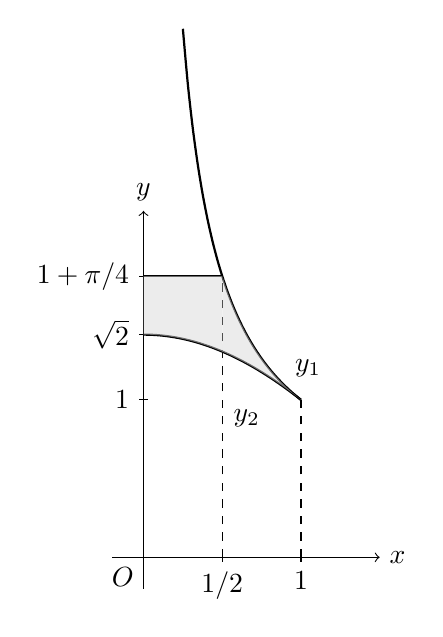
\begin{tikzpicture}[scale=2.0]
    \draw[->] (-0.2,0) -- (1.5,0) node[right]{$x$};
    \draw[->] (0,-0.2) -- (0,2.2) node[above]{$y$};
    \node[below left] at (0,0) {$O$};
    
    \draw (0.5,0.03) -- (0.5,-0.03) node[below]{$1/2$};
    \draw (1.0,0.03) -- (1.0,-0.03) node[below]{$1$};
    
    \draw (0.03,1.0) -- (-0.03,1.0) node[left]{$1$};
    \draw (0.03,1.414) -- (-0.03,1.414) node[left]{$\sqrt{2}$};
    \draw (0.03,1.785) -- (-0.03,1.785) node[left]{$1+\pi/4$};
    
    \draw[dashed] (0.5,0) -- (0.5, 1.785);
    \draw[dashed] (1.0,0) -- (1.0, 1.0);
    \draw[dashed] (0,1.785) -- (0.5, 1.785);
    
    \draw[thick, domain=0.25:1.0, smooth] plot (\x, {0.785398/\x - 0.785398 + 1});
    \node[right] at (0.9, 1.2) {$y_1$};
    
    \draw[thick, domain=0:1.0, smooth] plot (\x, {1.41421*cos(45*\x)});
    \node[below left] at (0.8, 1.0) {$y_2$};
    
    \draw[thick] (0,1.785) -- (0.5, 1.785);
    
    % Shading
    \fill[gray!30, opacity=0.5] (0,1.414) -- plot[domain=0:0.5, smooth] (\x, {1.41421*cos(45*\x)}) -- (0.5, 1.785) -- (0, 1.785) -- cycle;
    \fill[gray!30, opacity=0.5] (0.5, 1.156) -- plot[domain=0.5:1.0, smooth] (\x, {1.41421*cos(45*\x)}) -- (1.0, 1.0) -- plot[domain=1.0:0.5, smooth] (\x, {0.785398/\x - 0.785398 + 1}) -- cycle;
\end{tikzpicture}
\end{center}

\end{document}
